\section{Стабилизация программных движений двузвенного манипулятора без измерения скоростей.} \label{p22}

Вначале рассмотрим задачу о стабилизации программного положения горизонтального манипулятора без измерения скоростей в случае 

\begin{equation} \label{2.5'}
q^0_1 (t) = q^0_1 = const, \quad q^2_0 (t) = q^2_0 = const
\end{equation}

Эта задача в соответствии с представленным в параграфе 1.2 общим решением для голономной механической системы решается управлением вида 

\begin{equation} \label{2.6'}
\begin{array}{c}
\displaystyle U^{(1)}_1 (x_1) = - k_1 \sin \frac{x_1(t)}{2} - \int_{t-h}^t p_1^0 e^{s_1^0 (\tau - t)} (x_1 (t) - x_1 (\tau)) d \tau, \\ \displaystyle U^{(2)}_1 (x_1) = - k_2 \sin \frac{x_2(t)}{2} - \int_{t-h}^t p_2^0 e^{s_2^0 (\tau - t)} (x_2 (t) - x_2 (\tau)) d \tau
\end{array}
\end{equation}

$k_1, \ k_2, \ p_1^0, \ p_2^0, \ s_1^0, \ s_2^0 - const$

При этом, согласно теореме каждое возмущенное движение будет неограниченно приближаться при $t \to \infty$ к положению равновесия, определяемое равенствами 

$$\sin \frac{x_1(t)}{2} = 0 \quad \sin \frac{x_2(t)}{2} = 0$$

или $x_1(t) = 2 \pi k, \quad x_2(t) = 2 \pi k, \quad k \in Z$

Соответственно в переменных $q_1$ и $q_2$ для каждого возмущенного движения имеем при $t \to +\infty$ 

\begin{equation}
q_1 (t) \to q_1^0 + 2 \pi k, \quad q_2(t) \to q_2^0 + 2 \pi k
\end{equation}


Таким образом, так как положение манипулятора в переменных $q_1$ и $q_2$ определяются с точностью до $2 \pi,$ управлением (\ref{2.6'}) достигается глобальная стабилизация положения (\ref{2.5'}).

Выражение для кинетической энергии не содержит координату $q_1$ в явном виде, т.е. она является циклической. Вводим циклический импульс $$\frac{\partial T}{\partial \dot q_1} = a_{11} \dot q_1 + a_{12} \dot q_2 = v$$

Составим функцию Рауса. Для этого находим $\dot q_1 = (v - a_12 \dot q_2) / a_{11}$
$$
\begin{array}{c}
\displaystyle R = \frac12 (v - a_{12} \dot q_2)^2 / a_{11} + a_{22} (v - a_{12} \dot q_2) \dot q_2 / a_{11} + \frac12 a_{22} \dot q_2^2 - v (v - a_{12} \dot q_2) / a_{11} =\\
\displaystyle = \frac12 (a_{22} - a_{12}^2 / a_{11}) \dot q_2^2 - \frac12 v^2 / a_{11} + a_{12} v \dot q_2 / a_{11}
\end{array}
$$

Отсюда имеем следующие уравнения движения в переменных $q_2, \ \dot q_2, v$
$$\frac{d}{dt} ((a_{22} - a_{12}^2 / a_{11}) \dot q_2) - \frac12 \frac{\partial a_{11}}{\partial q_2} v_0^2 / a_{11}^2 = M_1$$
$$v = v_0 = const$$

Эти уравнения допускают движения вида 

\begin{equation}
v = v_0 = const, \quad \dot q_2 = 0, \quad q_2 = q_2^0 = const
\end{equation}

если 
$$U_1^0 = m_2 l l_2 \sin q_2^0 v_0^2 / (m_2 l^2 + I_1 + I_2 + 2 m_2 l l_2 \cos q_2^0)^2$$

В соответствии с представленным в параграфе 2.3 общим решением в задаче о стабилизации установленного движения голономной механической системы с циклической координатой получаем, что задача о стабилизации движения (2.2.4) по $q_2$ и $\dot q_2$ решается управлением
$$
\begin{array}{c}
\displaystyle U_2 = U_2^0 - k_2 \sin x_2 (t) - \int_{t-h}^{t} p_2^0 e^{s_2^0 (\tau - t)} (x_2 (t) - x_2 (\tau)) d \tau\\
\displaystyle k_2 = \frac{m_2 l l_2 \cos q_2^0 v_0^2}{(m l^2 + I_1 + I_2 + 2 m_2 l l_2 \cos q_2^0)^2}; \quad p_2^0, \quad s_2^0 - const > 0
\end{array}
$$

может быть достигнута также стабилизацией движения (2.2.4) по $p, \dot q_2$ и $q_2.$

\begin{figure}[h]
	\centering
	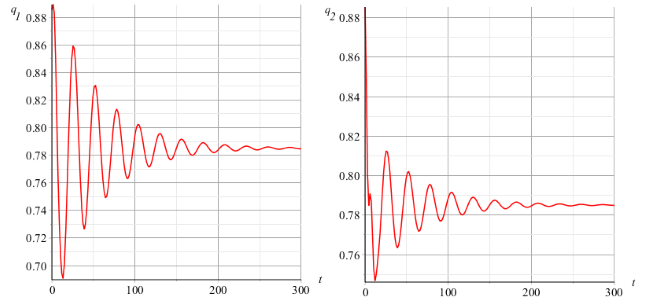
\includegraphics{horizontal}
	\caption{Результаты моделирования при управлении (2.6)}
	\label{fig:manip_horizontal}
\end{figure}

\begin{figure}[h]
	\centering
	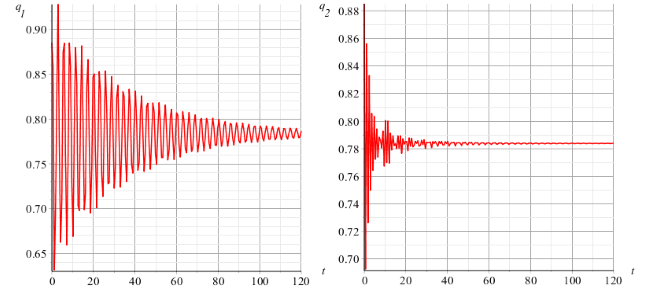
\includegraphics{vertical}
	\caption{Результаты моделирования при управлении (2.6)}
	\label{fig:manip_vertical}
\end{figure}

Рассмотрим задачу о стабилизации заданного программного положения вертикального двузвенного манипулятора. Из уравнений движения (2.2.3) находим, что положение (2.2.1) будет иметь место управление $$U_1^0 = -(m_1 l_1 + m_2 l_2) g \cos q_1^0, \quad U_2^0 = -m_2 l_2 g \cos (q_1^0 + q_2^0)$$

В соответствии в параграфе 1.2 общим решением получаем, что задачи о стабилизации программного положения (2.2.1) без измерения скоростей решается управлением 
$$
\begin{array}{l}
\displaystyle U_1 = U_1^0 - k_1 (q_1(t) - q_1^0) - \int_{t-h}^{t} p_1^0 e^{s_1^0 (\tau - t)} (q_1(t) - q_1(\tau)) d \tau\\
\displaystyle U_2 = U_2^0 - k_2 (q_2(t) - q_2^0) - \int_{t-h}^{t} p_2^0 e^{s_2^0 (\tau - t)} (q_2(t) - q_2(\tau)) d \tau
\end{array}
$$

где коэффициенты $k_1$ и $k_2$ удовлетворяет условиям 
$$
\begin{array}{c}
\alpha_1 k_1 - (m_1 l_1 + m_2 l) g \sin q_1^0 - m_2 l_2 g \sin (q_1^0 + q_2^0) > 0\\
\alpha_1 (k_2 - m_2 l_2 g \sin (q_1^0 + q_2^0)) - (m_2 l_2 g \sin (q_1^0 + q_2^0))^2 > 0
\end{array}
$$